% \section{Методы}
% \section{Сравнение возможных решений}
\section{Алгоритм работы программы}
\subsection{Представление задачи в терминах MapReduce}
Для параллельного запуска приложений была выбрана модель распределённых
вычислений MapReduce по ряду причин. Основные понятия:

Как оказалось задача без особых сложностей выражается в терминах
чистых функций flat map и flat reduce, так как основная структура,
используемая в алгоритме --- это пара(шаблон, количество совпадений)
и благодаря этому однопоточный код легко запускается
на множестве узлов MapReduce-кластера. Это обстоятельство освобождает
от реализации сложного механизма сетевого взаимодействия.

В качестве реализации модели MapReduce была выбрана реализация
Yandex Tables, обладающая рядом отличий и нововведений:
\begin{itemize}
  \item Колоночное хранение и range-операции
  \item Дерево метаинформации
  \item Единая операция Map-Reduce
  \item Расширенная поддержка транзакций, включая вложенность
  \item Настраиваемый коэффициент репликации и алгоритмы сжатия данных
  \item Хранение файлов в системе и их раздача исполняемым задачам
  \item Разные форматы стриминга (yamr, dsv)
  \item Надёжность и производительность
    \begin{itemize}
      \item Отказоустойчивый мультимастер
      \item Отказоустойчивый реплицированный планировщик
      \item Минорные обновления проходят без заметного эффекта для
        конечных пользователей
    \end{itemize}
  \item Гибкие слоты (заказ CPU, RAM)
  \item Существенные обновления не требуют пересборки C++ клиентов
    (так как все работает через HTTP API и стриминг клиент)
\end{itemize}
Не смотря на существенные отличия от модели, описанной в документе от компании
Google, код программы, реализующий алгоритм легко переносится
на другие реализации данной модели распределённых вычислений.

\subsection{Структура данных}
В качестве входных данных использовался агрегированный файл журнала с
нерегулярной структурой, содержащий сообщения об ошибках в различных форматах,
как многострочные, так и однострочные.

Первая часть алгоритма, позволяет осуществить сбор статистики
и возвращает список пар (шаблон, количество совпадений), так же существует
возможность получить часть текста не удовлетворяющую известным шаблонам,
для последующего анализа с помощью второй части алгоритма, позволяющей
выделить новые предполагаемые шаблоны и с помощью первой части алгоритма
получить статистику, подтверждающую или опровергающую предположение.

\subsection{Алгоритм}
На рисунке \ref{fig:algo} представлена упрощённая схема алгоритма подсчёта
количества совпадения шаблонов в терминах модели MapReduce.

\begin{figure}[h]
  \centering
  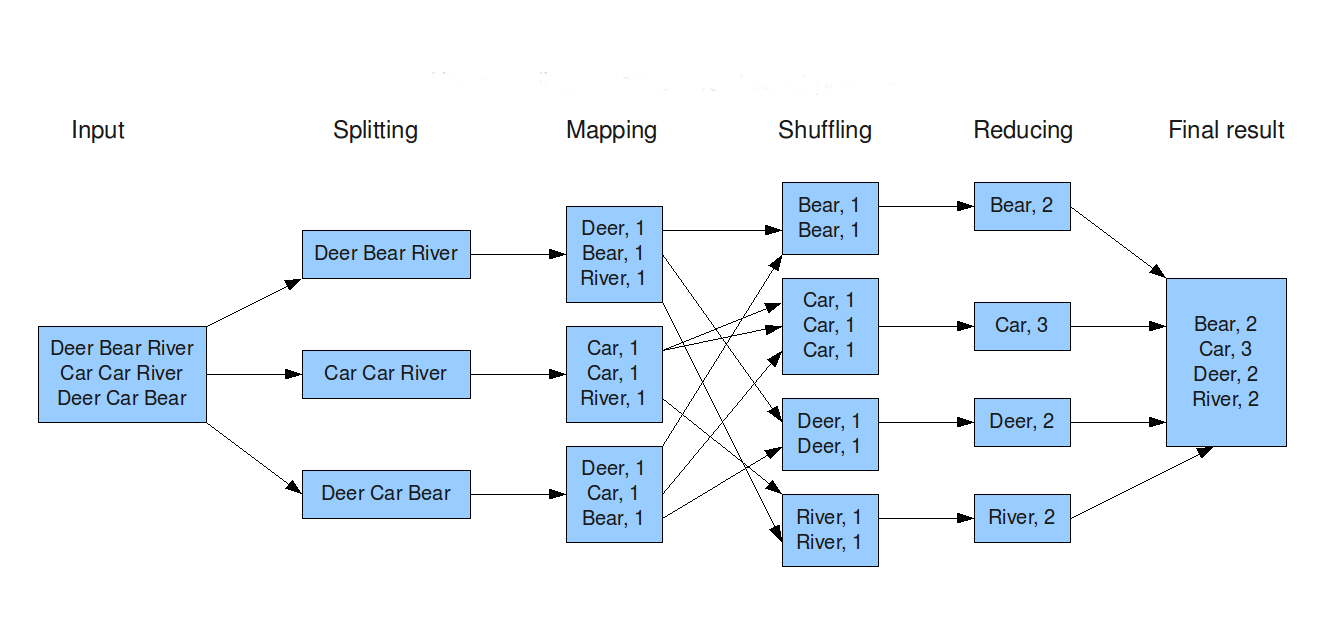
\includegraphics[width=\textwidth]{pics/mapreduce.png}
  \caption{Алгоритм подсчёта количества совпадений шаблонов}
  \label{fig:algo}
\end{figure}

На первом этапе(Splitting) происходит разбиение агрегированного файла журнала
на части и перемещение частей в оперативную память рабочих узлов
MapReduce-кластера.

На втором этапе(Mapping), в рамках каждого рабочего узла, происходит подсчёт
количества совпадений каждого шаблона.

На третьем этапе(Shuffling) происходит перераспределение данных между рабочими
узлами. Информация про одни и те же шаблоны попадают на один узел.

На четвёртом этапе(Reduce) происходит объединения информации про один шаблон.

На заключительном, пятом этапе, происходит генерация отчёта и запись его на
распределённую файловую систему.

\section{Особенности реализации, проблемы и способы их решения}

\subsection{Выбор языка программирования и средств разработки}
В качестве среды разработки было решено использовать удалённую виртуальную
машину с конфигурацией и окружением идентичными конфигурации и окружению
MapReduce узла. Были выбраны следующие программные продукты:

\begin{itemize}

\item В качестве операционной системы использовался дистрибутив\\ GNU/Linux
  Ubuntu 12.04 LTS с модифицированным ядром и дополнительными пакетами. Но
  принципиального отличия при использование приложения на официальном
  дистрибутиве возникнуть не должно.

\item Vim --- один из немногих настоящих текстовых редакторов,
  обладающих массой встроенных возможностей и практически безграничным
  потенциалом к расширению за счёт встроенного интерпретируемого языка
  программирования VimL и поддержкой возможности написания расширений на
  таких языках, как python, ruby, perl.

\item Сохранение состояние рабочего окружения осуществлялось с помощью
  терминального мультиплексора tmux, имеющего клиент-серверную архитектуру и
  позволяющего отсоединятся от текущей сессии, оставляя её работать в фоновом
  режиме с последующей возможностью переподключения.
  tmux --- свободная консольная утилита-мультиплексор,
  предоставляющая пользователю доступ к нескольким терминалам в рамках
  одного экрана. tmux может быть отключён от экрана: в этом случае он
  продолжит исполняться в фоновом режиме; имеется возможность вновь
  подключиться к tmux, находящемуся в фоне. tmux является штатным
  мультиплексором терминалов операционной системы OpenBSD.
  Программа tmux задумывалась как замена программы GNU Screen.

\item Удалённое подключение осуществлялось средствами защищённого протокола
ssh\\
(беспарольная аутентификация с использованием ключа) и технологии cauth.
SSH (англ. Secure Shell --- ``безопасная оболочка'']) --- сетевой протокол
прикладного уровня, позволяющий производить удалённое управление операционной
системой и туннелирование TCP-соединений (например, для передачи файлов).
Схож по функциональности с протоколами Telnet и rlogin, но, в отличие от них,
шифрует весь трафик, включая и передаваемые пароли. SSH допускает выбор
различных алгоритмов шифрования. SSH-клиенты и SSH-серверы доступны для
большинства сетевых операционных систем.

\item Для управления версиями исходных кодов использовалась децентрализованная
  система управления версиями git, в качестве сервиса для хранения репозитория
  был использован сервис github.

\end{itemize}

В качестве языка программирования был выбран python2.7. Так как:

\begin{itemize}
\item Он предустановлен в большинстве современных дистрибутивах
  операционных систем.
\item Выразителен. Аналогичные программы на таких языках как Java, C++
  имеют в разы большие объёмы исходных кодов.
\item Обладает высокой производительностью.
\item Имеет множество библиотек, в том числе библиотеки для работы с
  регулярными выражениями, обёртки для MapReduce.

\end{itemize}


\subsection{Подготовка репозитория}
Был создан git-репозиторий на сервисе github, сделана его локальная копия.
Была выбрана следующая структура проекта и правила именования файлов:

\begin{itemize}
\item В корневом каталоге лежат файлы README.md, LICENSE, .gitignore.
\item В каталоге doc/ хранится документация. Исходные тексты в \LaTeX и
  скомпилированная версия в PDF.
\item В каталоге direlog/ хранятся исходные коды с расширением .py и тесты,
  имеющие префикс test\_
\item В каталоге direlog/example/ хранятся примеры файлов журналов и
  вспомогательные скрипты на языке bash.
\end{itemize}

\subsection{Выбор хранилища для шаблонов}
В качестве хранилища для паттернов было решено использовать обычный файл на
языке python, названный patterns.py и содержащий в себе два списка паттернов
prepare\_patterns и main\_patterns, используемых на подготовительном этапе
и на этапе сбора статистики соответственно,
и хранить его под контролем версий в этом же репозитории. Причин
на это несколько: во-первых простота модификации файла с помощью скриптов,
во-вторых возможность просмотра истории изменений и откат к предыдущим версиям,
в-третьих возможность ручного редактирования.

\subsection{Написание программного кода}

Для разработки приложения, реализующего алгоритм была использована одна из
гибких методологий разработки - экстремальное программирование.\\

Использовались следующие приёмы этой методологии разработки:

\begin{itemize}
  \item Короткий цикл обратной связи
    \begin{itemize}
      \item Разработка через тестирование
      \item Заказчик всегда рядом
      \item Парное программирование
    \end{itemize}
  \item Непрерывный, а не пакетный процесс
    \begin{itemize}
      \item Непрерывная интеграция
      \item Рефакторинг
      \item Частые небольшие релизы
    \end{itemize}
  \item Понимание, разделяемое всеми
    \begin{itemize}
      \item Простота
      \item Коллективное владение кодом
      \item Стандарт кодирования
    \end{itemize}
    \item Социальная защищённость программиста
      \begin{itemize}
        \item 40-часовая рабочая неделя
      \end{itemize}
\end{itemize}

В результате можно выделить следующие этапы развития приложения:\\

\begin{enumerate}
\item Написание функциональных тестов для prepare.py.
\item Написание утилиты для предварительной обработки исходного файла журнала.
  Утилита получила название prepare.py и позволила подготовить сырой файл
  журнала для последующей обработки, путём замены уникальных токенов, таких
  как UUID, timestamp, версии, номера строк, пути, содержащие версии, на
  строковые константы.
\item Формирование prepare\_patterns на основе ручного анализа
  файлов журналов.
\item Написание функциональных тестов для direlog.py.
\item Реализация алгоритма для сбора статистики с использованием\\
  main\_patterns. Утилита получила название direlog.py. И позволяет на
  выходе получить список пар (шаблон, количество совпадений) или текст,
  не подходящий под известные шаблон.
\item Написание функциональных тестов для direlog.py.
\item Добавление поддержки буферизации входного потока и поддержки
  многострочных шаблонов.
\item Добавление функции, позволяющей запускать алгоритм на MapRedcue-кластере.
\end{enumerate}

Для сбора файлов журналов используется приложение collect-logs.py,
представленное в приложении Д, в котором используется коммерческая технология
skynet. При использовании данного приложения в среде, где отсутствует
вышеупомянутая технология стоит использовать такие альтернативы как rbtorrent
или rsync.


